\sectionSlide{C++ future}{binario}{\paperwidth}{b}


\timeSlide{C++17}{
    \begin{itemize}
        \item std::variant
        \item if constexpr(expression)
        \item auto in templates
        \item structured bindings
        \item if and switch with initializer
        \item many, many more...
    \end{itemize}
}{    
    \draw[thin,blue]
    (0.5, 0) node(l1979)[anchor=west] {1979 C with Classes}
    (0.5,-0.4) node(l1981)[anchor=west] {1981 New features}
    (0.5,-0.7) node(l1983)[anchor=west] {1983 1st std lib}
    (0.5,-1.0) node(l1984)[anchor=west] {1984 C84/C++ }
    (0.5,-1.3) node(l1985)[anchor=west] {1985 Cfront 1.0}
    (0.5,-1.6) node(l1989)[anchor=west] {1989 Cfront 2.0}
    (0.5,-2.0) node(l1991)[anchor=west] {1991 Cfront 3.0}
    (0.5,-2.4) node(l1993)[anchor=west] {1993 Cfront 4.0}
    (0.5,-3.2) node(l1998)[anchor=west] {1998 C++98}
    (0.5,-4.0) node(l2003)[anchor=west] {2003 C++03}
    (0.5,-5.0) node(l2011)[anchor=west] {2011 C++11}
    (0.5,-5.5) node(l2014)[anchor=west] {2014 C++14}
    (0.5,-6.0) node(l2017)[anchor=west,fill=green!20,rounded corners] {\textbf{2017} C++17};
    
    \draw[]
    (1979) -- (l1979)
    (1981) -- (l1981)
    (1983) -- (l1983)
    (1984) -- (l1984)
    (1985) -- (l1985)
    (1989) -- (l1989)
    (1991) -- (l1991)
    (1993) -- (l1993)
    (1998) -- (l1998)
    (2003) -- (l2003)
    (2011) -- (l2011)
    (2014) -- (l2014)
    (2017) -- (l2017);
}


\slide{C++17}{
    \begin{itemize}
        \item Michael Wong - C++17, Will It Be Great Or Just OK
        \item Many planned features are out of scope
        \item Backward compatibility hamper the standardization of new features
        \item Stackoverflow list of C++17 features \footnotemark
    \end{itemize}
    \footnotetext[3]{\url{http://stackoverflow.com/questions/38060436/what-are-the-new-features-in-c17}}
}


\timeSlide{C++20}{
    \centering
    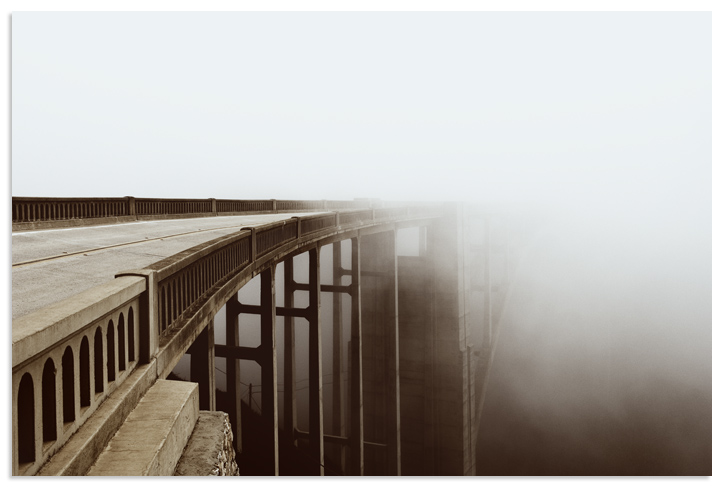
\includegraphics[height=0.8\paperheight]{unknown-future}
}{    
    \draw[thin,blue]
    (0.5, 0) node(l1979)[anchor=west] {1979 C with Classes}
    (0.5,-0.4) node(l1981)[anchor=west] {1981 New features}
    (0.5,-0.7) node(l1983)[anchor=west] {1983 1st std lib}
    (0.5,-1.0) node(l1984)[anchor=west] {1984 C84/C++ }
    (0.5,-1.3) node(l1985)[anchor=west] {1985 Cfront 1.0}
    %(0.5,-2.0) node(l1986)[anchor=west] {1986 Cfront 1.1}
    %(0.5,-2.4) node(l1987)[anchor=west] {1987 Cfront 1.2}
    (0.5,-1.6) node(l1989)[anchor=west] {1989 Cfront 2.0}
    %(0.5,-3.2) node(l1990)[anchor=west] {1990 Cfront 2.1}
    (0.5,-2.0) node(l1991)[anchor=west] {1991 Cfront 3.0}
    (0.5,-2.4) node(l1993)[anchor=west] {1993 Cfront 4.0}
    (0.5,-3.2) node(l1998)[anchor=west] {1998 C++98}
    (0.5,-4.0) node(l2003)[anchor=west] {2003 C++03}
    (0.5,-5.0) node(l2011)[anchor=west] {2011 C++11}
    (0.5,-5.5) node(l2014)[anchor=west] {2014 C++14}
    (0.5,-6.0) node(l2017)[anchor=west] {2017 C++17}
    (0.5,-6.5) node(l2020)[anchor=west,fill=green!20,rounded corners] {\textbf{2020} C++20};
    
    \draw[]
    (1979) -- (l1979)
    (1981) -- (l1981)
    (1983) -- (l1983)
    (1984) -- (l1984)
    (1985) -- (l1985)
    %(1986) -- (l1986)
    %(1987) -- (l1987)
    (1989) -- (l1989)
    %(1990) -- (l1990)
    (1991) -- (l1991)
    (1993) -- (l1993)
    (1998) -- (l1998)
    (2003) -- (l2003)
    (2011) -- (l2011)
    (2014) -- (l2014)
    (2017) -- (l2017)
    (2020) -- (l2020);
}


\slide{C++ future - summary}{
    \itemstep{
        \item C++17 is almost ready
        \item Future version are planned to be released every 3 years
        \item Next planned version: C++20 (minor)
        \item Backward compatibility hamper the standardization of new features
        \item gcc and clang already support many of C++17 features
        \item MSVC is behind them
    }
}